\section{Adatbázisséma}

Az adatbázisséma tervezéséhez a dbdiagram.io nevű platformfüggetlen, webes ER diagram tervező szoftvert használtam.
Ez egy saját fejlesztésű, DBML nevű DSL nyelvet használ a séma leírására, és lehetővé teszi ennek exportálását különféle formátumokba.

\begin{figure}[!ht]
\centering
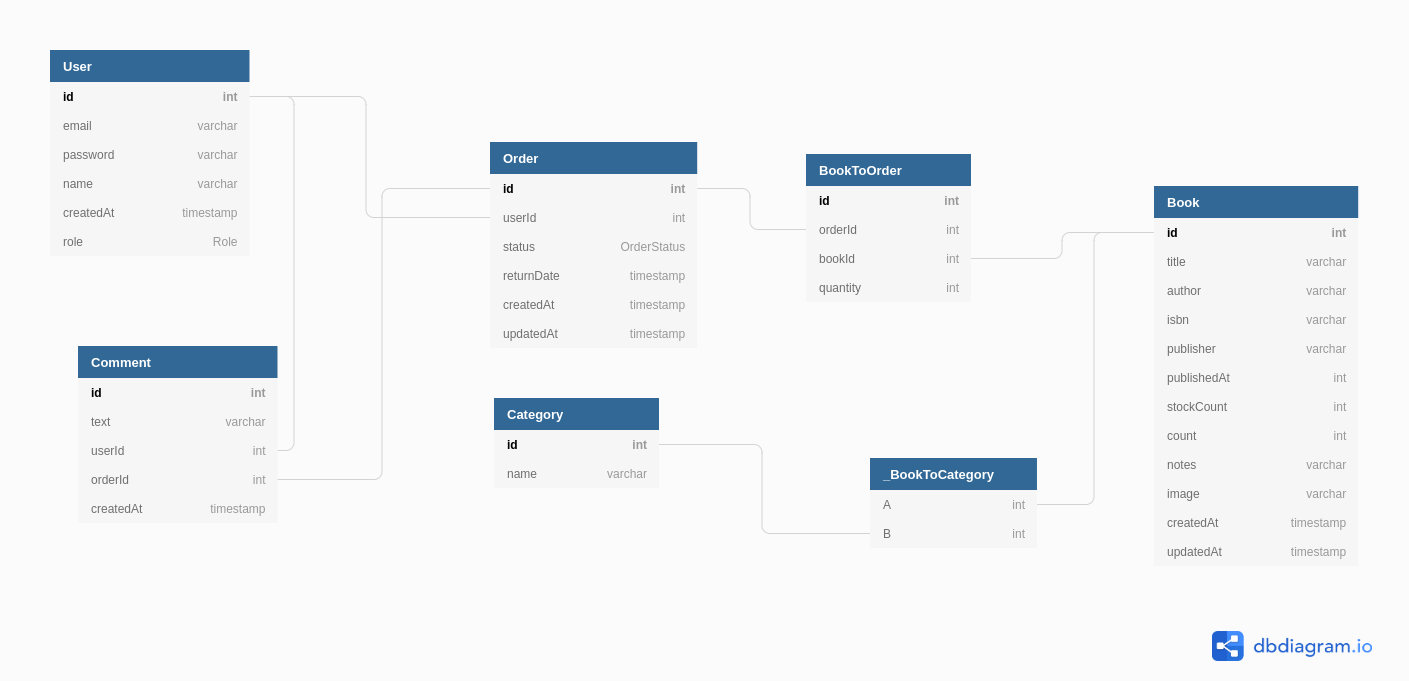
\includegraphics[width=150mm, keepaspectratio]{figures/dbschema.png}
\caption{Az adatbázisséma ER diagramja.}
\label{fig:DBSchema}
\end{figure}

A séma tervezése során a Prisma által használt elnevezési konvenciókat használtam megkönnyítve a két technológia közötti átjárhatóságot.
